\documentclass{article}[11pt]
\usepackage{fullpage,graphicx, setspace, latexsym, cite,amsmath,amssymb,xcolor,subfigure}
%\usepackage{epstopdf}
%\DeclareGraphicsExtensions{.pdf,.eps,.png,.jpg,.mps} 
\usepackage{amssymb} %maths
\usepackage{amsmath} %maths
\usepackage{amsthm, comment}
\usepackage[round,comma,sort,numbers, compress]{natbib}

% \bibliographystyle{plain}
\bibliographystyle{plos2015}

\newtheorem{theorem}{Theorem}
\newtheorem{prop}{Proposition}
\newtheorem{corollary}{Corollary}
\newtheorem{lemma}{Lemma}
\newtheorem{defn}{Definition}
\newtheorem{ex}{Example}
\usepackage{float}

\newcommand*{\underuparrow}[1]{\underset{\uparrow}{#1}}
\usepackage{graphicx}
\usepackage{xcolor}
\usepackage[dvipsnames]{xcolor}
\usepackage{algorithmicx}
\usepackage{algorithm} %http://ctan.org/pkg/algorithms
\usepackage{algpseudocode} %http://ctan.org/pkg/algorithmicx
\usepackage{enumitem}
\usepackage{simplemargins}
\usepackage{hyperref}
\hypersetup{
     colorlinks=true,
     linkcolor=blue,
     filecolor=red,
     citecolor = red,      
     urlcolor=cyan,
}

\usepackage{mdframed}
\definecolor{lgray}{rgb}{0.92,0.92,0.92}
\definecolor{lsalmon}{rgb}{0.9921568627450981,0.9411764705882353, 0.9254901960784314}

\renewcommand{\bibnumfmt}[1]{#1.}
\setlist{noitemsep} % or \setlist{noitemsep} to leave space around whole list
\setallmargins{1in}
\linespread{1.1}

\newcommand{\brows}[1]{%
  \begin{bmatrix}
  \begin{array}{@{\protect\rotvert\;}c@{\;\protect\rotvert}}
  #1
  \end{array}
  \end{bmatrix}
}
\newcommand{\rotvert}{\rotatebox[origin=c]{90}{$\vert$}}
\newcommand{\rowsvdots}{\multicolumn{1}{@{}c@{}}{\vdots}}


\def\R{\mathbb{R}}
\def\Eps{\mathcal{E}}
\def\E{\mathbb{E}}
\def\V{\mathbb{V}}
\def\F{\mathcal{F}}
\def\G{\mathcal{G}}
\def\H{\mathcal{H}}
\def\S{\mathcal{S}}
\def\D{\mathcal{D}}
\def\P{\mathbb{P}}
\def\1{\mathbf{1}}
\def\n{\nappa}
\def\h{\mathbf{w}}
\def\v{\mathbf{v}}
\def\x{\mathbf{x}}
\def\X{\mathcal{X}}
\def\Y{\mathcal{Y}}
\def\eps{\epsilon}
\def\y{\mathbf{y}}
\def\e{\mathbf{e}}
\newcommand{\norm}[1]{\left|\left|#1\right|\right|}
\DeclareMathOperator*{\argmin}{arg\,min}
\DeclareMathOperator*{\argmax}{arg\,max}
\newcommand{\lecture}[4]{
   \pagestyle{myheadings}
   \thispagestyle{plain}
   \newpage
   % \setcounter{lecnum}{#1}
   \setcounter{page}{1}
   \setlength{\headsep}{10mm}
   \noindent
   \begin{center}
   \framebox{
      \vbox{\vspace{2mm}
    \hbox to 6.28in { {\bf CHEME 5820: Machine Learning for Engineers
   \hfill Spring 2025} }
       \vspace{4mm}
       \hbox to 6.28in { {\Large \hfill Lecture #1: #2  \hfill} }
       \vspace{2mm}
       \hbox to 6.28in { {\it Lecturer: #3 \hfill #4} }
      \vspace{2mm}}
   }
   \end{center}
   \markboth{Lecture #1: #2}{Lecture #1: #2}

   \noindent{\bf Disclaimer}: {\it These notes have not been subjected to the
   usual scrutiny reserved for formal publications. }
   \vspace*{4mm}
}

\begin{document}
\lecture{6a}{Incorportaing Gene Expression into the Flux Bounds}{Jeffrey Varner}{}

\begin{mdframed}[backgroundcolor=lgray]
    In this lecture, we will discuss the following topics:
    \begin{itemize}[leftmargin=16pt]
      \item{Flux balance analysis (FBA) is a mathematical approach used to analyze the flow of metabolites through a metabolic network. It assumes a steady state where metabolite production, consumption, and transport rates are balanced. The FBA problem is formulated as a linear programming (LP) problem to maximize or minimize fluxes through the network, subject to constraints and bounds.}
      \item{\href{sec-material-balance}{Material balance constraints} are used to ensure that the flow of metabolites into and out of a system is balanced (and physical). These constraints are typically represented as a set of linear equations, where the coefficients represent the stoichiometry of the reactions in the system in combination with transport and dilution terms.}
      \item{\href{sec-flux-bounds}{Flux bounds constraints} limit the range of possible fluxes through a metabolic network. These bounds can incorporate additional information, such as experimental data or prior knowledge about the system, into the FBA problem.}
    \end{itemize}
 \end{mdframed}

\section{Introduction}
In this lecture, we dive deeper into the material balance constraints and the flux bounds in the 
flux balance analysis (FBA) framework. In particular, we will discuss incorporating gene expression data into the flux bounds.

\section{Material Balance Constraints}\label{sec-material-balance}
Flux balance analysis (FBA) aims to estimate intracellular reaction rates (fluxes) using available experimental data.
The more available data, the more constraints we can put on the system, the more accurate our flux estimates will be.
However, one of the powerful aspects of FBA is that it can estimate metabolic fluxes even for systems with little data.
Suppose we have a system with a species set $\mathcal{M}$, stream set $\mathcal{S}$, and a reaction set $\mathcal{R}$. 
Further, suppose that the system (or at least part of it) is at or near a steady state. 
The optimal reaction rates can be estimated using the following linear program (Defn. \ref{defn-fba-concentration}).
\begin{mdframed}
\begin{defn}[Flux Balance Analysis Problem)]\label{defn-fba-concentration}
The flux balance analysis problem, whose solution provides estimates for the values of the unknown fluxes, is the linear program: 
\begin{align*}
\max_{\hat{v}}\quad&  \sum_{i\in\mathcal{R}}c_{i}\hat{v}_{i}\\
\text{subject to}\quad & \sum_{s\in\mathcal{S}}d_{s}C_{i,s}\dot{V}_{s} + \sum_{j\in\mathcal{R}}\sigma_{ij}\hat{v}_{j}V = \frac{d}{dt}\left(C_{i}V\right)\qquad\forall{i\in\mathcal{M}}\\
& \mathcal{L}_{j}\leq\hat{v}_{j}\leq\mathcal{U}_{j}\qquad\forall{j\in\mathcal{R}}
\end{align*}
Here, $\sigma_{ij}$ are elements of the stoichiometric matrix $\mathbf{S}$, $c_{i}$ are objective coefficients (you choose), $\hat{v}_{i}$ are unknown fluxes, and $\mathcal{L}_{j}$ and $\mathcal{U}_{j}$ are the lower and upper flux bounds, respectively.
The $d_{s}$ terms are the direction parameters for the streams, and the $\dot{V}_{s}$ terms are the volumetric flow rates for the streams. 
\end{defn}
\end{mdframed}
However, this formulation looks slightly different from the one in Orth et al. \cite{Orth:2010aa}.
Let's explore this further.

\subsection{Simplified Species Constraints}
In the Orth et al. primer \cite{Orth:2010aa}, the material balance constraints were written as $\mathbf{S}\hat{\mathbf{v}} = 0$. 
This is a simplification; in reality, the material balance constraints are more complex. But let's see how we get there.
When doing FBA, we often will make three assumptions:
\begin{itemize}[leftmargin=16pt]
\item{\textbf{Steady-state, constant volume}: The biological system (or at least part of it) is in a steady state, and in whole-cell models, the volume of the culture is constant. However, this is not the case in fed-batch cultures; many industrial biotechnology processes operate in fed-batch mode.}
\item{\textbf{Specific units}: The volume basis for the intracellular species concentrations is in specific units, i.e., per unit cell mass measured in grams dry weight (units: gDW). For cell-free systems, the volume basis is the volume of the reaction.}
\item{\textbf{No transport or dilution terms}: We will assume that there are no physical transport or dilution terms in the material balance equations. This is a simplification, but it is often used in FBA. For example, this assumption is not the case for continuous cell-free systems.}
\end{itemize}

\subsubsection*{Derivation of the Palsson Constraints}
Let the volume of our system be written in specific units, i.e., $V=B\bar{V}$, where $B$ is the biomass concentration (units: gDW/L) and $\bar{V}$ is the volume of the culture (units: L). 
The material balance constraints can be simplified by assuming the species in our system are in a steady state. 
But there is more to this story. Let's expand the accumulation terms:
\begin{align*}
\frac{d}{dt}\left(C_{i}V\right) &= \frac{d}{dt}\left(C_{i}B\bar{V}\right)\\
&= B\bar{V}\underbrace{\left(\frac{dC_{i}}{dt}\right)}_{\text{steady state}\,=\,0} + C_{i}B\underbrace{\left(\frac{d\bar{V}}{dt}\right)}_{\text{steady state\,=\,0}} + C_{i}\bar{V}\left(\frac{dB}{dt}\right)\\
C_{i}\bar{V}\left(\frac{dB}{dt}\right) & = \underbrace{\sum_{s\in\mathcal{S}}d_{s}C_{i,s}\dot{V}_{s}}_{\text{no transport\,=\,0}} + \sum_{j\in\mathcal{R}}\sigma_{ij}\hat{v}_{j}V\\
C_{i}\bar{V}\left(\frac{dB}{dt}\right) & = \sum_{j\in\mathcal{R}}\sigma_{ij}\hat{v}_{j}B\bar{V}\\
C_{i}\underbrace{\left[\frac{1}{B}\left(\frac{dB}{dt}\right)\right]}_{\text{specific growth rate $\mu$}} & = \sum_{j\in\mathcal{R}}\sigma_{ij}\hat{v}_{j}\\
C_{i}\mu & = \sum_{j\in\mathcal{R}}\sigma_{ij}\hat{v}_{j}\\
\sum_{j\in\mathcal{R}}\sigma_{ij}\hat{v}_{j} - \underbrace{C_{i}\mu}_{\text{small}\,\ll{1}} & = 0\\
\sum_{j\in\mathcal{R}}\sigma_{ij}\hat{v}_{j} & = 0\quad\forall{i\in\mathcal{M}}\quad\blacksquare
\end{align*}


\subsubsection*{Exchange Reactions}
Great! So then, does everything in our system have to be at a steady state? Not exactly. 
We can think of the system we are studying as an open system, i.e., it can exchange material with the 
surroundings. Thus, while the components of the system are in a steady state, the universe (system + surroundings) 
as a whole is not. This is a subtle point, but it is essential to understand. The exchange of material with the
surroundings is captured in the context of our three assumptions by writing hypothetical reactions that 
exchange material with the surroundings. We call these reactions the \texttt{exchange reactions}.
Consider the toy network in Fig. \ref{fig:example-exchange-reactions}.
The exchange reactions are written as those that cross the system's boundary.

\begin{figure}
   \centering
 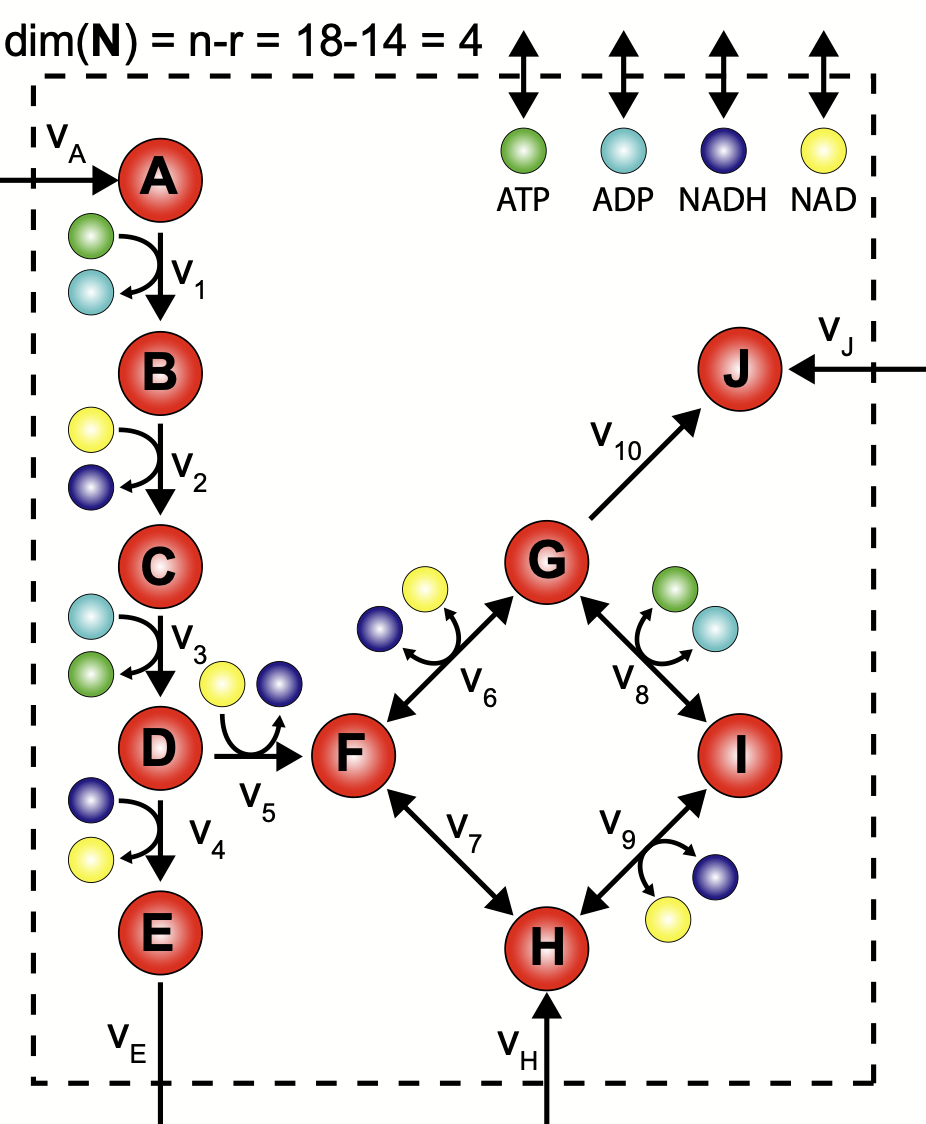
\includegraphics[width=0.44\textwidth]{./figs/Fig-ExchangeReactions.png}
 \caption{Example network reproduced from Bordbar et. al., \citep{Bordbar:2014aa}.
 The exchange reactions cross the boundary of the system. We have (potentially) enzyme-catalyzed 
 exchanges, e.g., $\left\{v_{A},v_{E}, v_{H}, v_{J}\right\}$ and hypothetical exchanges, e.g., ATP or NADH.}\label{fig:example-exchange-reactions}
\end{figure}


\section{Flux Bounds}\label{sec-flux-bounds}
The flux bounds are essential constraints in flux balance analysis calculations and the convex decomposition of the stoichiometric array. 
Beyond their role in the flux estimation problem, the flux bounds are integrative. These constraints integrate many types of genetic and biochemical information into the problem. 
A general model for these bounds is given by:
\begin{align*}
-\delta_{j}\underbrace{\left[{V_{max,j}^{\circ}}\left(\frac{e}{e^{\circ}}\right)\theta_{j}\left(\dots\right){f_{j}\left(\dots\right)}\right]}_{\text{reverse: other functions or parameters?}}\leq\hat{v}_{j}\leq{V_{max,j}^{\circ}}\left(\frac{e}{e^{\circ}}\right)\theta_{j}\left(\dots\right){f_{j}\left(\dots\right)}
\end{align*}
where $V_{max,j}^{\circ}$ denotes the maximum reaction velocity (units: flux) computed at some characteristic enzyme abundance. 
Thus, the maximum reaction velocity is given by:
\begin{equation*}
V_{max,j}^{\circ} = k_{cat,j}^{\circ}e^{\circ}
\end{equation*}
where $k_{cat,j}$ is the catalytic constant or turnover number for the enzyme (units: 1/time) and $e^{\circ}$ is a characteristic enzyme abundance (units: concentration). 
The term $\left(e/e^{\circ}\right)$ is a correction to account for the actual enzyme abundance catalyzing the reaction (units: dimensionless). 
The $\theta_{j}\left(\dots\right)\in\left[0,1\right]$ is the current fraction of maximial enzyme activity of enzyme $e$ in reaction $j$. 
The activity model $\theta_{j}\left(\dots\right)$ describes \href{https://en.wikipedia.org/wiki/Allosteric_regulation}{allosteric effects} on the reaction rate, 
and is a function of the regulatory and chemical state of the system, the concentration of substrates, products, and cofactors (units: dimensionless).
Finally, the $f_{j}\left(\dots\right)$ is a function describing the substrate (reactants) dependence of the reaction rate $j$ (units: dimensionless). 

\subsection{Simplfied bounds model}
Let's initially assume that $(e/e^{\circ})\sim{1}$, there are no allosteric inputs $\theta_{j}\left(\dots\right)\sim{1}$, and the substrates are saturating $f_{j}\left(\dots\right)\sim{1}$. 
Then, the flux bounds are given by:
\begin{align*}
-\delta_{j}V_{max,j}^{\circ}\leq{\hat{v}_{j}}\leq{V_{max,j}^{\circ}}
\end{align*}
This is a simple model for the flux bounds. 
It is easy to see that the flux bounds are a function of the maximum reaction velocity, the catalytic constant or turnover number, and our assumed value of a characteristic enzyme abundance.

\subsection{Turnover numbers and reversiblity}
The turnover number, $k_{cat}$, measures an enzyme's catalytic activity, defined as the number of substrate molecules converted to product per enzyme molecule per unit time. Units are typically 1/time (e.g., 1/s or 1/min). 
Values can be obtained from primary literature or databases like \href{https://www.brenda-enzymes.org/}{BRENDA} \citep{BRENDA2021}.
The second thing we need to estimate is the reversibility parameter.
The reversibility parameter $\delta_{j}$ can be computed in several ways. For example, one method in the literature is to use the sign of Gibbs reaction energy:
\begin{equation*}
\delta_{i} = \begin{cases}
0 & \text{if }\text{sign}\left(\Delta{G}^{\circ} - \Delta{G}^{\star}\right)= -1 \quad\text{irreversible} \\
1 & \text{if }\text{sign}\left(\Delta{G}^{\circ} - \Delta{G}^{\star}\right)= +1 \quad\text{reversible}
\end{cases}
\end{equation*}
where $\Delta{G}^{\circ}$ is the standard Gibbs free energy change of the reaction, and $\Delta{G}^{\star}$ is a threshold value (hyperparameter). 
The threshold value can be set to zero or some other value. Alternatively, the value of $\delta_{j}$ can be assigned based upon a cutoff $K^{\star}$ on the equilibrium constant:
\begin{equation*}
\delta_{i} = \begin{cases}
0 & \text{if }K_{eq}>\,K^{\star}\quad\text{irreversible} \\
1 & \text{if }K_{eq}\leq\,K^{\star}\quad\text{reversible}
\end{cases}
\end{equation*}
where you specify the value $K^{\star}$ based upon some intution or other criteria. We can compute the $\Delta{G}^{\circ}$ values using \href{ttps://equilibrator.weizmann.ac.il}{eQuilibrator} \citep{Beber:2022aa}.

\section{Gene expression models}
One of the shortcomings that we discussed about flux balance analysis was: 
FBA may conflict with experimental data, especially when regulatory loops are excluded. 
These discrepancies reveal the limitations of relying only on stoichiometric information without considering complex cellular regulation. 
This can be (partially) fixed by including gene expression in the bounds.
Gene expression is easy(ish), but allosteric regulation (activity) is hard.

Let's investigate how we could describe gene regulation in flux balance analysis. 
Suppose the flux problem we were interested in was composed of enzymes encoded by the genes $\mathcal{G}=1,2,\dots, N$.
The action of each gene is described by two differential equations, one for mRNA concentration ($m_{j}$, units: nmol/gDW) 
and a second for the corresponding protein concentration ($p_{j}$, units: nmol/gDW):
\begin{align*}
	\dot{m}_{j} &= r_{X,j}u_{j}\left(\dots\right) - \left(\theta_{m,j}+\mu\right)\cdot{m_{j}}+\lambda_{j}\quad{j=1,2,\dots,N}\\
	\dot{p}_{j} &= r_{L,j}w_{j}\left(\dots\right) - \left(\theta_{p,j}+\mu\right)\cdot{p_{j}}
\end{align*}
Terms in the balances:
\begin{itemize}[leftmargin=16pt]
\item{\textbf{Transcription}: The term $r_{X,j}u_{j}\left(\dots\right)$ in the mRNA balance denotes the regulated rate of transcription for gene $j$. This is 
the product of a kinetic limit $r_{X,j}$ (units: nmol/gDW-time) and a transcription control function $0\leq{u_{j}\left(\dots\right)}\leq{1}$ (dimensionless).
The final term $\lambda_{j}$ is the unregulated expression rate of mRNA $j$ (units: nmol/gDW-tim`), i.e., the leak expression rate.}
\item{\textbf{Translation}: The regulated rate of translation of mRNA $j$, denoted by $r_{L,j}w_{j}$, is also the product of the
kinetic limit of translation (units: nmol/gDW-time) and a translational control term $0\leq{w_{j}\left(\dots\right)}\leq{1}$ (dimensionless).}
\item{\textbf{Degradation}: Lastly, $\theta_{\star,j}$ denotes the first-order rate constant (units: 1/time) governing degradation of protein and mRNA, and $\mu$ 
is the specific growth rate of the cell (units: 1/time). We get the latter term using cell-specific concentration units (e.g., nmol/gDW).}
\end{itemize}

\subsection{Steady-state gene expression}
We have publically said (without proof yet) that gene expression is slow and metabolism is fast. Suppose this is true.
This means that the mRNA and protein concentrations are at an approximate steady state, i.e., $\dot{m}_{j}=\dot{p}_{j}=0$ from the perspective of the metabolic network. 
This allows us to solve the gene expression equations for the steady-state mRNA and protein concentrations. 
Let's show the steps to compute the steady-state mRNA concentration $m^{\star}_{j}$:
\begin{align*}
r_{X,j}u_{j}\left(\dots\right) - \left(\theta_{m,j}+\mu\right)\cdot{m_{j}}+\lambda_{j} & = \dot{m}_{j}\\
r_{X,j}u_{j}\left(\dots\right) - \left(\theta_{m,j}+\mu\right)\cdot{m^{\star}_{j}}+\lambda_{j} &= 0 \\
r_{X,j}u_{j}\left(\dots\right) + \lambda_{j} & = \left(\theta_{m,j}+\mu\right)\cdot{m^{\star}_{j}}\\
\frac{r_{X,j}u_{j}\left(\dots\right) + \lambda_{j}}{\theta_{m,j}+\mu} &= m^{\star}_{j}\quad\text{for }j=1,2,\dots,N\quad\blacksquare
\end{align*}
Following the same steps, we can compute the steady-state protein concentration $p^{\star}_{j}$:
\begin{equation*}
p^{\star}_{j} = \frac{r_{L,j}w_{j}\left(\dots\right)}{\theta_{p,j}+\mu}\quad\text{for }j=1,2,\dots,N\quad\blacksquare
\end{equation*}
Some things to think about:
\begin{itemize}[leftmargin=16pt]
\item{Nonlinearity: The expressions for $m^{\star}_{j}$ and $p^{\star}_{j}$ are tricker than they may seem at first blush. 
The steady-state mRNA and protein concentrations are a function of the kinetic limits of transcription and translation, the control functions, the degradation rates, and the specific growth rate of the cell. At the mRNA level, the $u(...)$ model could be a function of metabolite and protein concentrations. While the kinetic limit of translation $r_{L,j}$ and the $w_{j}(...)$ terms will be functions of the mRNA concentrations and other factors, 
such as ribosome availability, etc.}
\item{Models: We need to formulate the control functions $u_{j}(...)$ and $w_{j}(...)$, and the degradation rates $\theta_{m,j}$ and $\theta_{p,j}$, and the kinetic limits $r_{X,j}$ and $r_{L,j}$ for each gene in the system. 
These will be functions of parameters that must be estimated from literature studies or experimental data.}
\item{Complication: Finally, the enzymes catalyzing the reactions in the metabolic network are often complexes of different protein subunits, where a different gene encodes each subunit. We need to formulate the gene-protein-reaction (GPR) rules that link the genes to the proteins and the proteins to the reactions in the metabolic network. 
This will allow us to integrate the gene expression logic into the flux balance analysis problem.}
\end{itemize}

\section{Summary}
This lecture discussed the material balance constraints and the flux bounds in the flux balance analysis (FBA) framework.
The material balance constraints ensure that the flow of metabolites into and out of a system is balanced, 
while the flux bounds limit the range of possible fluxes through a metabolic network.
These constraints and bounds are essential for estimating the intracellular reaction rates using FBA and integrating genetic and biochemical information into the problem.
We developed some simple models for modeling gene expression and incorporating gene expression data into the flux bounds.
This will allow us to incorporate gene expression control into the FBA problem and improve the accuracy of our flux estimates.

\bibliography{References-W5.bib}

\end{document}